\chapter{設計}\label{chap:design}

本章では、本研究で提案するプログラミング環境の設計について述べる。

\section{設計指針}\label{ux8a2dux8a08ux6307ux91dd}

第\ref{chap:background}章では、計算資源としての人間についての考察を述べ、
人間と計算機の処理を融合させた新しいプログラミング環境の必要性について述べた。
現状の仕組みでは、既存のプログラミング言語上で具体的な人物を対象とした、
人間と計算機の融合型のプログラムを記述・実行することはできない。
本章ではこのプログラミング環境の設計と検討を行う。

特定の人物を計算機と同じようにプログラムから利用出来るようにするためには以下の要素が必要である。

\begin{itemize}
\itemsep1pt\parskip0pt\parsep0pt
\item
  プログラム上での対象人物の指定
\item
  プログラムから人への処理内容の伝達
\item
  人からプログラムへの処理結果の伝達
\item
  記法の検討
\end{itemize}

また、人間とプログラムのインタフェースとして機能するソフトウェアが必要となる。
このソフトウェアは、様々なデバイスや既存ソフトウェア上で動作させることが出来れば有用である。
この際、デバイスごとに仕様が異なる可能性や、
既存ソフトウェア上で動かす場合は、そのソフトウェアの仕様に沿った実装をしなくてはいけないという点を考慮する必要がある。
インタフェースとなるソフトウェアを実装しやすくするために、外部の仕様に左右されやすい部分を
換装が容易に可能なモジュールとして設計する。
これらの点について、以下の節にて詳しく設計を述べる。

\section{プログラムと人間のインタラクション設計}\label{sec:program-human-interaction-design}

\subsection{プログラムと人間のメッセージ交換モデル}\label{ux30d7ux30edux30b0ux30e9ux30e0ux3068ux4ebaux9593ux306eux30e1ux30c3ux30bbux30fcux30b8ux4ea4ux63dbux30e2ux30c7ux30eb}

プログラムと人間のインタラクションを実現するためには、
プログラムと人間がメッセージを交換できるようなモデルの構築が必要となる。
このモデルを構築するため、従来のプログラムとコンピュータの関係を応用する。

従来のコンピュータプログラムでは、書かれている処理を実行する対象はコンピュータである。
コンピュータはコンピュータプログラムに書かれている内容に忠実に従い、処理を行う。
これは、プログラムからの処理命令をコンピュータがメッセージとして受け取り、
そのメッセージの通りに処理を実行し、
その実行結果をプログラムに返すという、プログラムとコンピュータのメッセージ交換であると言える。

このモデルをそのままプログラムと人間の関係にも適応する。
つまり、プログラムからの処理命令を人間がメッセージとして受け取り、人間はそのメッセージ通りに処理を行う。
そして、実行した結果をプログラムに返す。
このメッセージ交換モデルを構築することが可能ならば、プログラムと計算機の間と同等のインタラクションを
プログラムと人間の間でも実現させることが出来る。

しかし現状では、プログラムから人間に直接メッセージを送る手法は存在せず、
人間からプログラムへと直接メッセージを送る手法も存在しない。
そこで、本研究においては、
インターネット接続していてメッセージを受信可能なデバイスを仲介することによって、
デバイス経由で人間にメッセージを送る。
つまり、デバイスを経由して指示内容を伝え、デバイスを経由して処理結果を入力させるという、
デバイス仲介型のプログラムと人間のメッセージ交換モデルを採用する。

このメッセージングモデルによって、プログラムと人間のコミュニケーションを実現する。

\subsection{具体的な人間の指定}\label{ux5177ux4f53ux7684ux306aux4ebaux9593ux306eux6307ux5b9a}

既存の仕組みでは、具体的な人物を指定し、プログラム上で計算資源として活用することはできない。
これは主に人間の知能に注目し、その能力を活かすことが既存の仕組みの目的であるからだ。
そのため、安価ですぐに多数の人を利用可能なクラウドソーシングを利用するほうが理にかなっており、
具体的な人間を指定する必要がなかった。

\begin{figure}[htbp]
  \begin{center}
  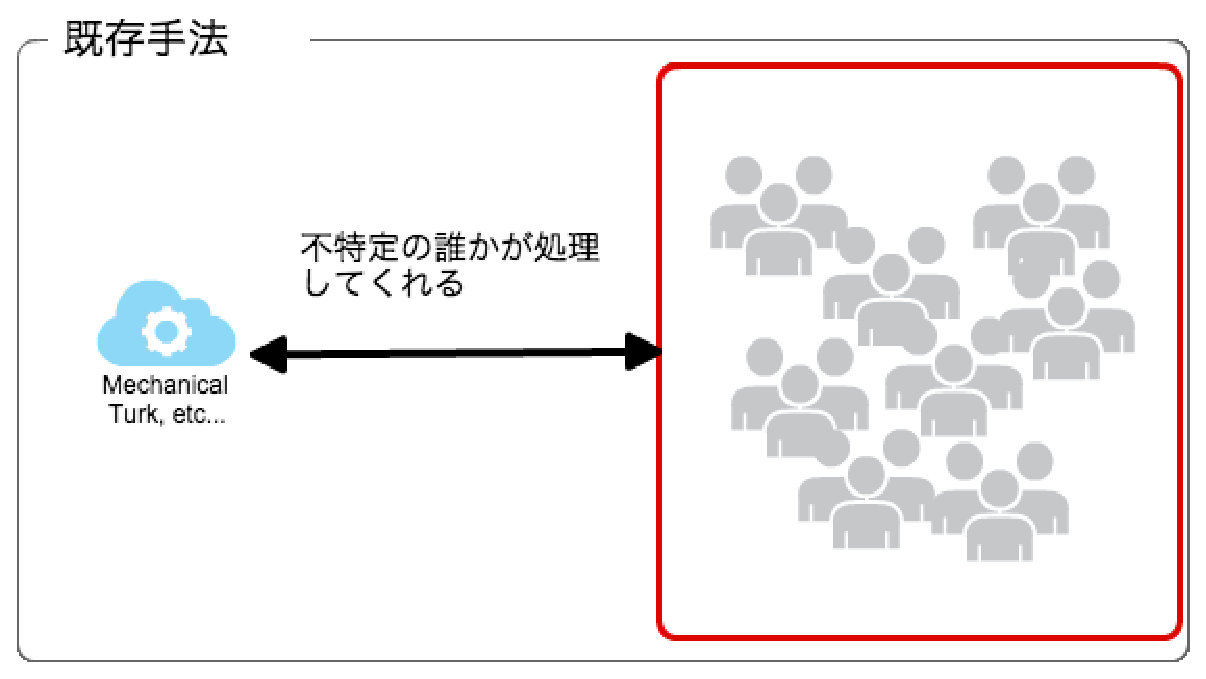
\includegraphics[width=.5\linewidth]{images/crowdsourcing_model.eps}
  \end{center}
  \caption{クラウドソーシングのモデル}
  \label{fig:crowdsourcing_model}
\end{figure}

しかし、本研究では人間の実世界のタスクの処理能力にも注目しているため、具体的な人物の指定が必要となる。
例えば、自分の家におけるタスクを処理するためには、自分や家族を指定する必要がある。
そこで、プログラム上で具体的な人間を宣言し、指示を送れるような仕組みを採用する。
このような仕組みを採用することで、プログラムと人間のメッセージングモデルにおいて具体的な人間の指定を可能にする。

\begin{figure}[htbp]
  \begin{center}
  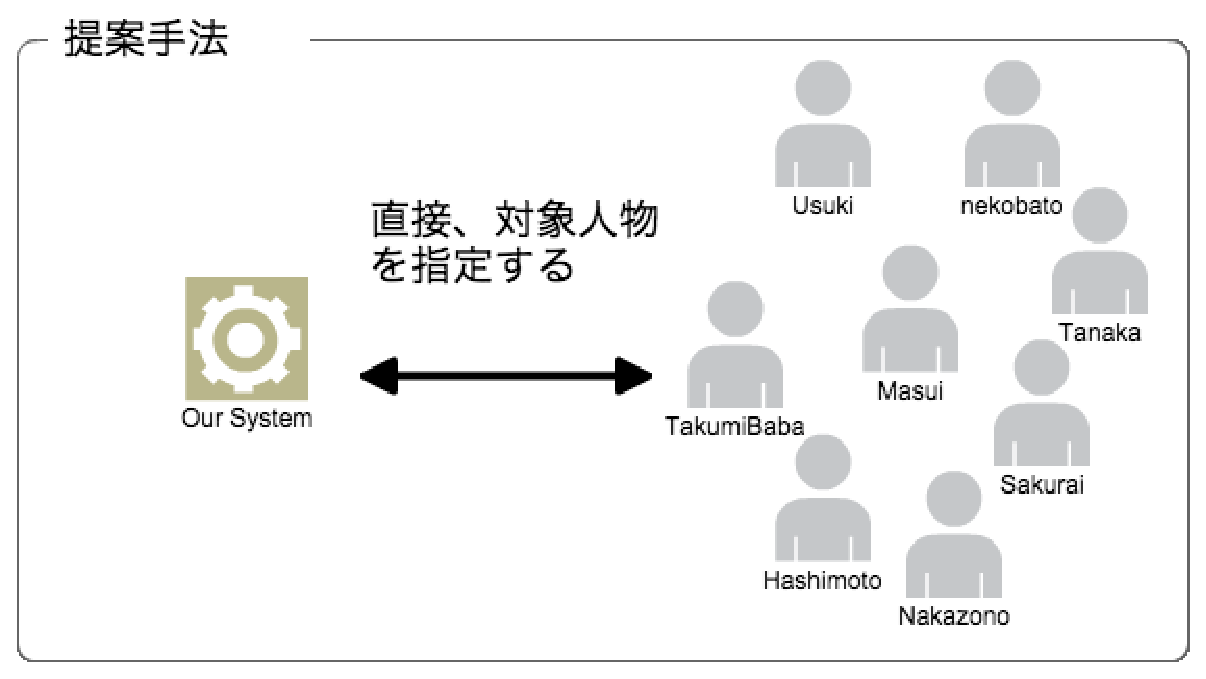
\includegraphics[width=.5\linewidth]{images/unique_id_model.eps}
  \end{center}
  \caption{提案手法のモデル}
  \label{fig:unique_id_model}
\end{figure}

\subsection{記法の検討}\label{ux8a18ux6cd5ux306eux691cux8a0e}

人間への指示を既存のプログラムと同じような記法で実現させる。
本研究では、人間と計算機を融合させることを目的としており、両者への指示が大きく異なることは避ける必要がある。
類似の記法で実現させ、状況に応じて両者の利用を自由に切り替えたりできるようにする必要がある。

例えば、データベースに問い合わせ、保存されているデータを取得するプログラムでの記述と同じような記法で
人間に問い合わせ、データを取得するようなプログラムが記述できるべきである。
データベースに情報があるならば、データベースに問い合わせる処理を実行すれば良いし、
ないならば、人間に問い合わせれば良い(ソースコード:\ref{code:design-integrated-program-style})。

\begin{lstlisting}[caption=人間への指示を計算機への指示と類似させる, label=code:design-integrated-program-style]
// データベース問い合わせの擬似コード
new db('tasks').find({id: 1}, function(err, doc){

});
// 人間への問い合わせの擬似コード
new Human('takumibaba').find({message: ''}, function(err, result){

});
\end{lstlisting}

同様に、センサーを利用して部屋の温度を取得するプログラムの記述と同じような記法で
人間を利用して、部屋のセンシングに利用するようなプログラムが記述できるべきだ。
センサーが部屋にないならば、人間に問い合わせれば良い。

これらの処理の切り替えを容易に記述できるようにするためには、可能な限り類似の記法を踏襲する必要がある。

\subsection{人間とプログラムのインタフェース}\label{ux4ebaux9593ux3068ux30d7ux30edux30b0ux30e9ux30e0ux306eux30a4ux30f3ux30bfux30d5ux30a7ux30fcux30b9}

前節までの設計に関する考察のように、人間とプログラムのメッセージングによって
両者のインタラクションを実現するためには、人間とプログラムのインタフェースとして機能するソフトウェアが必要である。
プログラムからの指示をユーザに提示し、処理を促し、何かしらの結果を入力するまでの一連の流れを担うものである。

必要な実装要件としては、以下の通りである。

\begin{itemize}
\itemsep1pt\parskip0pt\parsep0pt
\item
  指示内容の提示
\item
  実行結果の入力フォームの提示
\end{itemize}

上記内容、特に実行結果の入力フォームの提示における工夫をすることで、人間への負担を減らすように設計する必要がある。
まず、入力する情報の限定などが考えられる。
例えば、プログラム側で求めている結果が、Boolean型であるならばtrueかfalseを返すようなインタフェースのみを提示すべきである。
また、指示内容に従えない場合や現実との乖離から実行出来ない場合などに放置するということがないよう、
エラーを返すことのできるような仕組みを取り入れる必要がある。

このような、人間とプログラムの間を仲介するソフトウェアの実装は、人間とプログラムのインタラクションの実現に不可欠である。

\section{プラガブルなモジュール構成}\label{sec:plaggable-module-design}

様々なデバイスやソフトウェア上でプログラムと人間とのインタフェースを実装・運用する可能性がある。
だが、近年ではデバイスは多様化しており、その仕様も大きくことなる。
例えば、パソコンやスマートフォンではユーザに提示すべきインタフェースの設計が異なる。
画面の大きさの違いはそのままインタフェースの設計に影響を与える。
また、通信手法も異なることが多い。
パソコンであれば、基本的に常時コネクションを張り続けるといったことが可能であるが、スマートフォンの場合は
コネクションを切られてしまうこともある。

こういった状況を考慮して、デバイス依存しやすい部分については、交換が容易に可能なモジュールとして設計する必要がある。
交換可能なモジュールとして設計することで、デバイスごとに依存部分のプログラムを書くだけで、
共通部分の再実装をする必要がなくなる。
また、応用アプリケーション等の実装も容易となる、

本研究では、デバイス依存が強いと考えている以下の2点に関して、特別なモジュールとして扱う。

\begin{itemize}
\itemsep1pt\parskip0pt\parsep0pt
\item
  通信手法
\item
  ユーザインタフェース
\end{itemize}

通信手法は各デバイスごとに異なるため、選択可能であることが望ましい。
可能ならば、プログラムとデバイスが常にコネクションを貼り続け、いつでもリアルタイムに通信が出来る状態にしておくことが良いが、
リアルタイム通信が実現出来ない状況も存在する。
例えばスマートフォンの場合はOSによっては、一定時間の経過もしくはアプリケーションがバックグラウンド処理に回された際に
リアルタイム通信を切断をすることがある。
移動中等、通信状況が安定しない場合も考えられ、一つの通信手法に縛られず、様々な手法を利用できることが望ましい。

提示すべきユーザインタフェースも交換可能にしておくべきである。
スクリーンサイズの問題や、何かしらの既存ソフトウェア上に実装する場合には
ユーザインタフェースはその仕様に合うように提示すべきである。

また、上記の2点以外の部分に関しても、プラグインという形で拡張が可能になるような実装を行う。

\section{新しいプログラミング環境の要件のまとめ}\label{ux65b0ux3057ux3044ux30d7ux30edux30b0ux30e9ux30dfux30f3ux30b0ux74b0ux5883ux306eux8981ux4ef6ux306eux307eux3068ux3081}

前節までの設計検討から、人間と計算機への指示を融合させた新しいプログラミング環境の要件についてまとめる。
まず、\ref{sec:program-human-interaction-design}節をまとめると、以下の要素が必要となる。

\begin{itemize}
\itemsep1pt\parskip0pt\parsep0pt
\item
  プログラム上で人間とのインタラクションを可能にするプログラムモジュール
\item
  プログラムと人間の仲介となるソフトウェア
\end{itemize}

前者のプログラムモジュールは、具体的な人間を指定可能で、既存のプログラミングスタイルを踏襲して
人間への指示を送り、その実行結果を得ることが出来る。
後者では、指示に対して人間が値を返しやすいようなユーザインタフェースを提供し、
プログラムと人間の間の情報のやりとりをサポートする。

次に、\ref{sec:plaggable-module-design}節から、主にソフトウェアエージェントを運用するデバイスや
既存アプリケーションごとに異なる可能性の高い仕様の部分に関しては、容易に実装が可能で、交換できる
モジュールになるよう設計し、実装する。
拡張性を可能な限り高め、関連するプログラムの実装を容易にすることが目的である。

これらをまとめて、人間と計算への指示を融合させたプログラミング環境として提案する。
次章では、このプログラミング環境の各要素について詳しく述べる。
